\section{Experimental implementation}
\label{sec:experimental}



\begin{figure}[H]
    \centering
    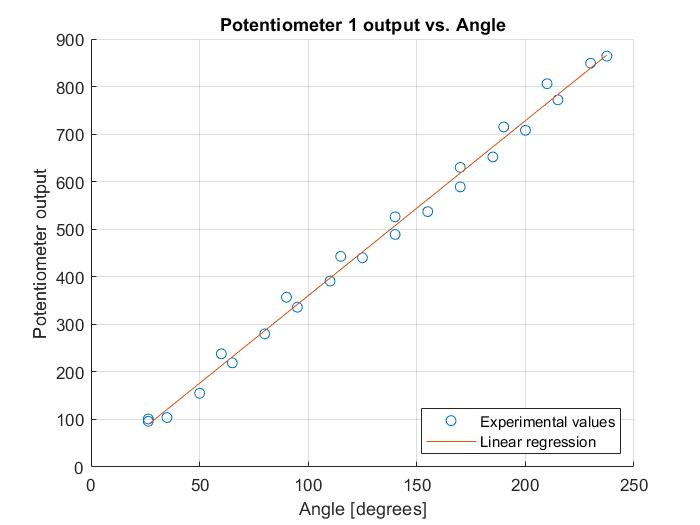
\includegraphics[width=0.7\textwidth]{figures/pot1.jpg}
    \caption{Relation between angle and potentiometer 1 output}
    \label{fig:pot1}
\end{figure}

\begin{align*}
    \begin{cases}
        y = 3.6806\,x  - 7.8262 \\
        R^2 = 0.9966
    \end{cases}
\end{align*}

\begin{figure}[H]
    \centering
    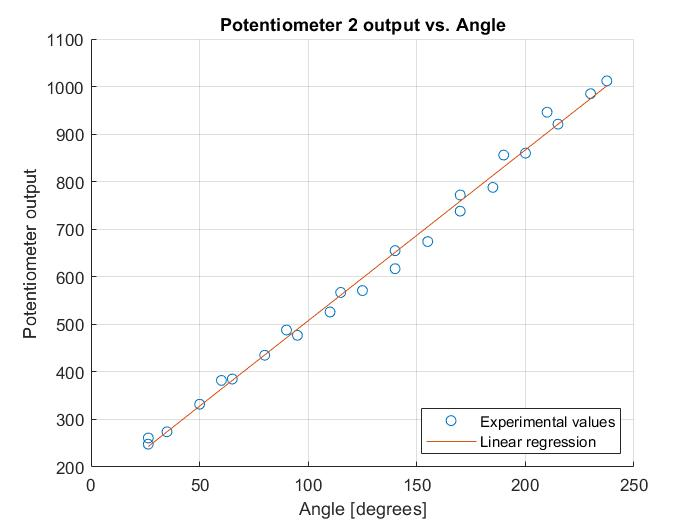
\includegraphics[width=0.7\textwidth]{figures/pot2.jpg}
    \caption{Relation between angle and potentiometer 2 output}
    \label{fig:pot2}
\end{figure}

\begin{align*}
    \begin{cases}
        y = 3.5921\,x + 148.3947 \\
        R^2 = 0.9969 
    \end{cases}
\end{align*}



\begin{figure}[H]
    \centering
   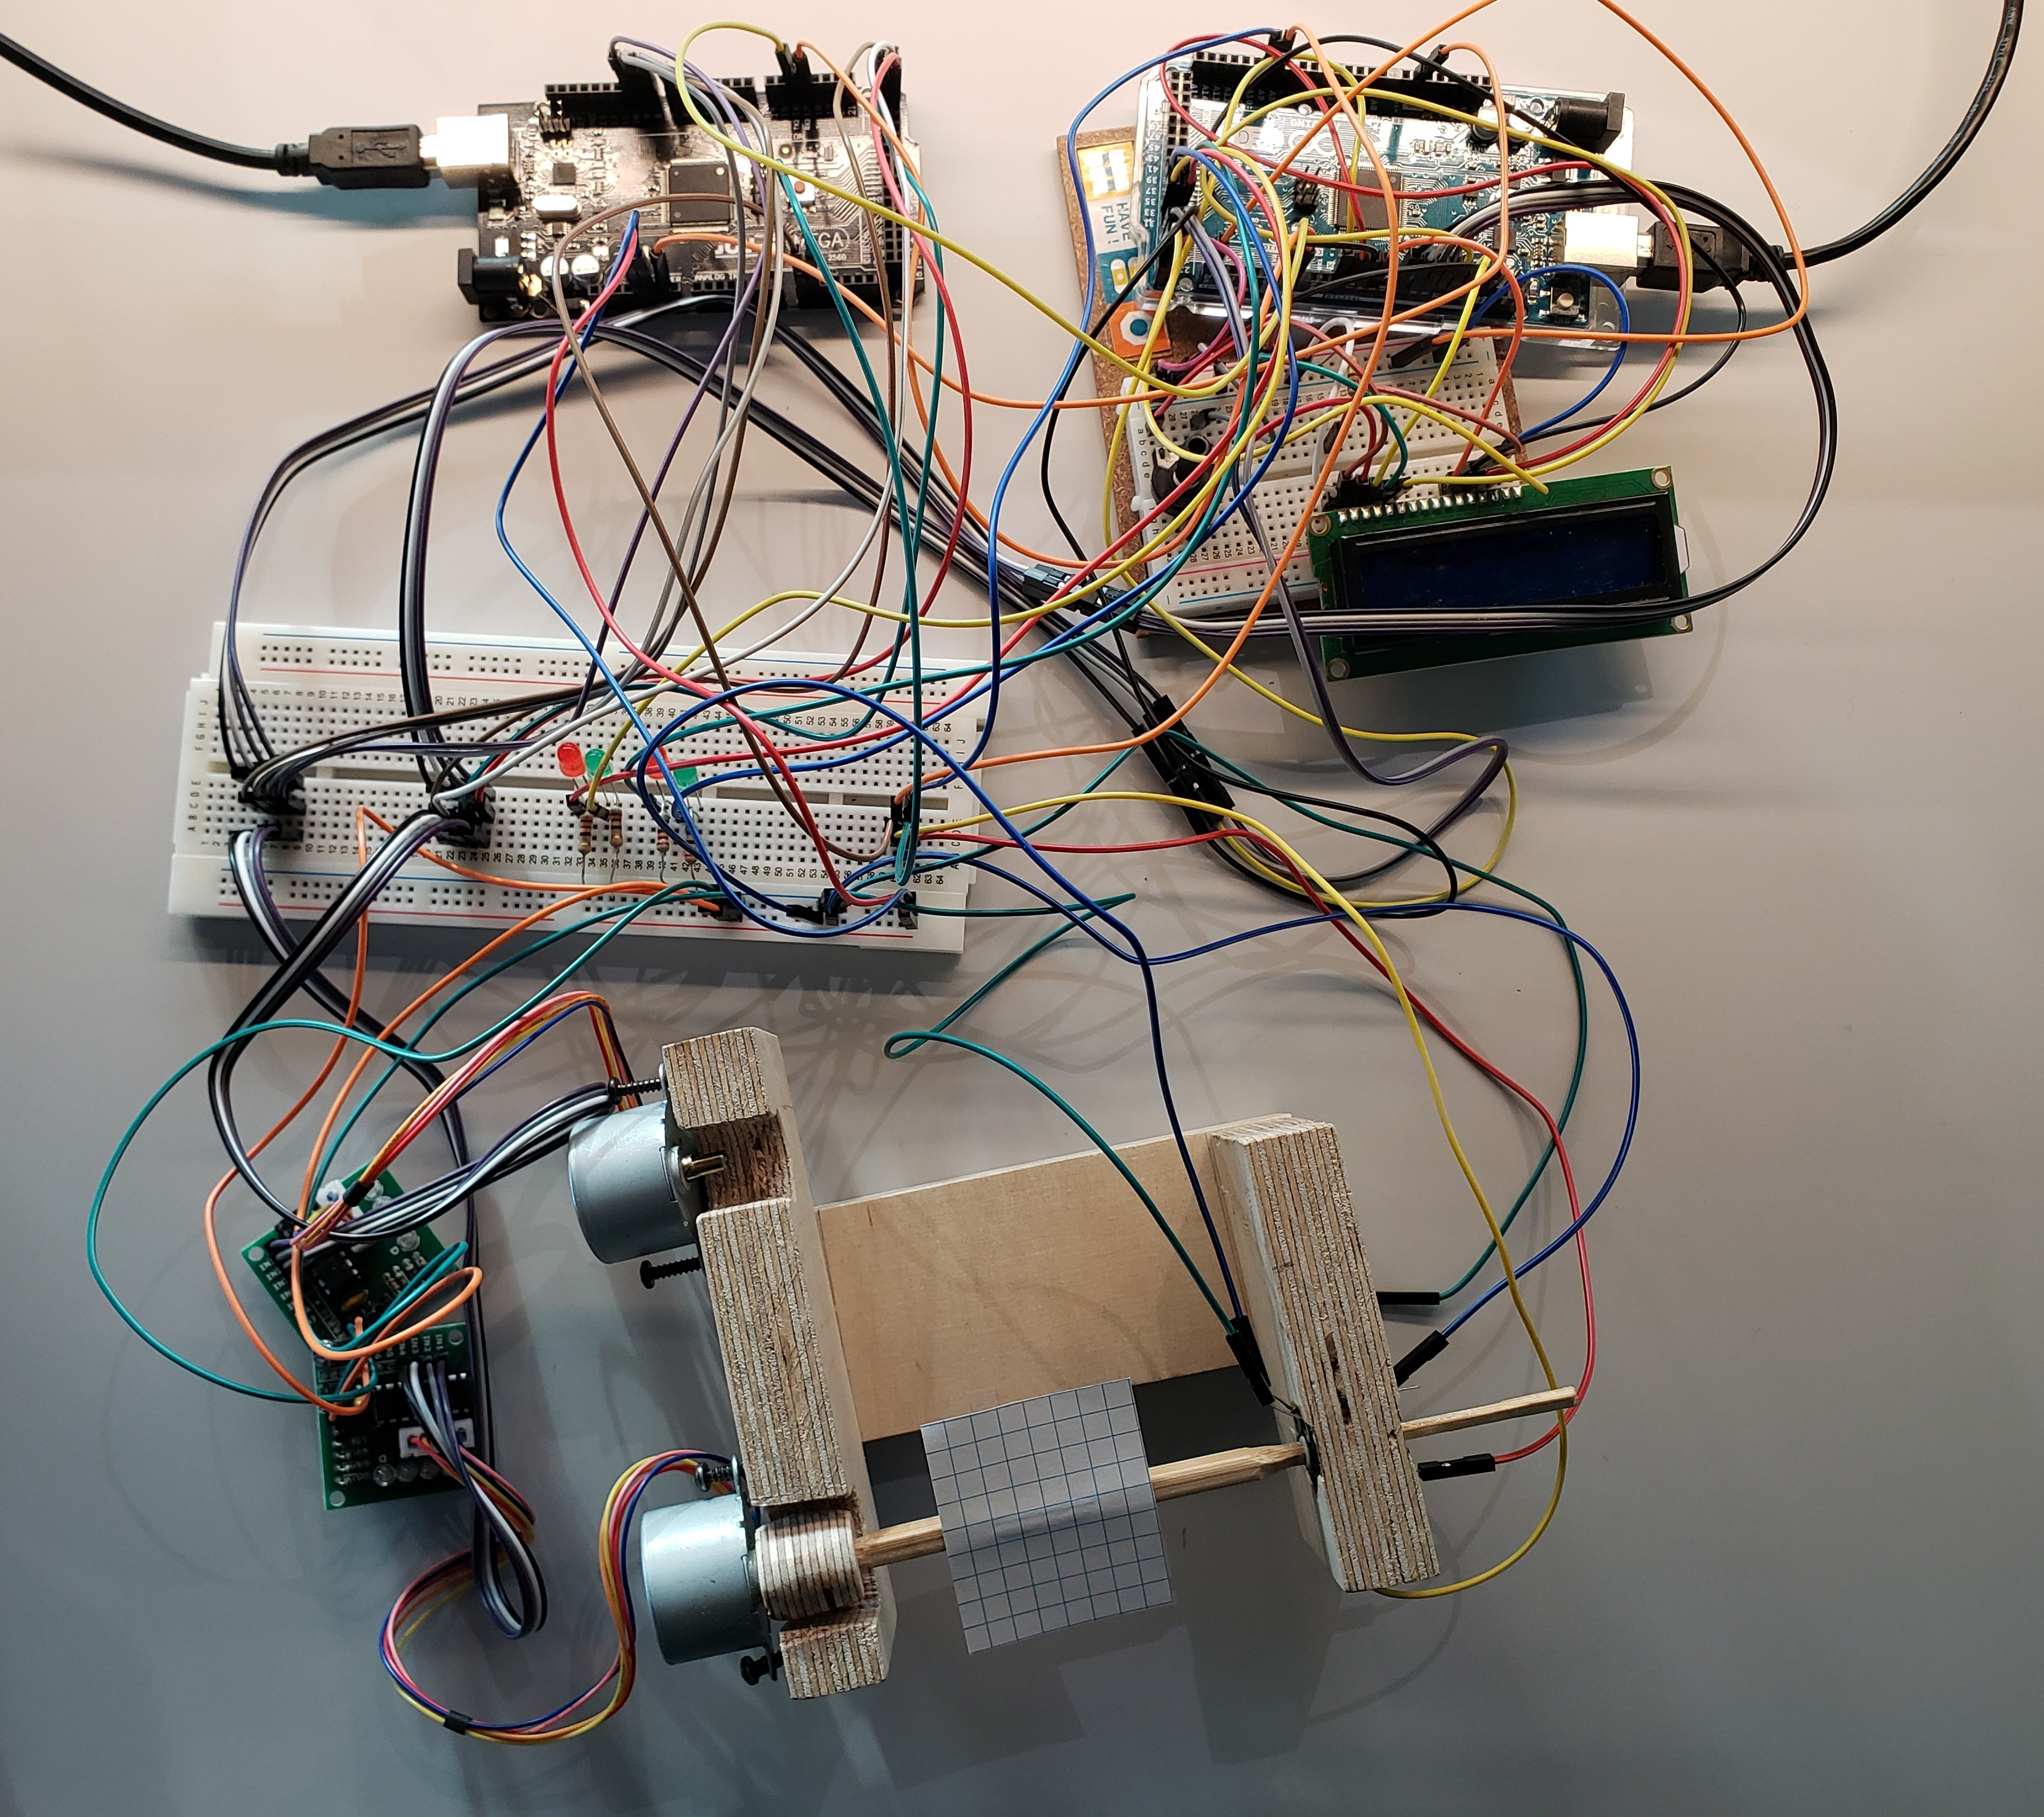
\includegraphics[width=\textwidth]{figures/circuit_pic.jpg}
    \caption{Circuit schematic}
     \label{fig:implented_design}
\end{figure}



add specific angle range that can be used